%% LyX 2.3.7 created this file.  For more info, see http://www.lyx.org/.
%% Do not edit unless you really know what you are doing.
\documentclass[english]{mwart}
\usepackage[T1]{fontenc}
\usepackage[latin9]{inputenc}
\usepackage{geometry}
\geometry{verbose,tmargin=2cm,bmargin=2cm,lmargin=2cm,rmargin=2cm,headheight=2cm,headsep=2cm,footskip=2cm}
\usepackage{babel}
\usepackage{graphicx}
\usepackage[unicode=true]
 {hyperref}
\begin{document}
\title{Raport cz\k{e}\'{s}ciowy z wykonanych prac w ramach umowy poz. 1/01/689/2024}
\author{Piotr Kalaczy\'{n}ski}
\maketitle

\section*{Szczeg�\l owy wykaz obowi\k{a}zk�w:}
\begin{enumerate}
\item Zebranie obraz�w z przejazd�w pojazd�w mechanicznych
\item Detekcja obiekt�w w pozyskanych danych
\item Wyznaczanie trajektorii dla poruszaj\k{a}cych si\k{e} obiekt�w
\item Por�wnanie problemu ze \'{s}ledzeniem cz\k{a}stek w detektorach
\item Opracowanie raportu
\end{enumerate}

\section{Dokumentacja:}

Ca\l y kod rozwijany w ramach wyznaczonych zada\'{n} przechowywany
jest w formie otwartej w repozytorium \href{https://github.com/pkalaczynski/automotive-tracking}{GitHub/pkalaczynski/automotive-tracking}.
Dokumentacja zawarta jest w pliku \href{https://github.com/pkalaczynski/automotive-tracking/blob/main/README.md}{README.md}.

\section{Post\k{e}p prac:}

Dotychczas wykonane zosta\l y nast\k{e}puj\k{a}ce zadania: 

\subsection{Zebranie obraz�w z przejazd�w pojazd�w mechanicznych:}

Zosta\l y zebrane zr�\.{z}nicowane obrazy z przejazd�w:
\begin{enumerate}
\item Dane z misji Apollo15: \href{https://archive.org/download/Apollo15And1616mmOnboardFilm}{https://archive.org/download/Apollo15And1616mmOnboardFilm}
\item Nagranie z drona pokazuj\k{a}ce drog\k{e} podmiejsk\k{a} w Houston:
\href{https://shorturl.at/gALOU}{https://shorturl.at/gALOU}
\end{enumerate}
Ponadto, dodana zosta\l a mo\.{z}liwo\'{s}\'{c} przetworzenia dowolnego
filmu dost\k{e}pnego w serwisie YouTube, np.:
\begin{enumerate}
\item Nagranie z przejazdu w \'{s}r�dmie\'{s}ciu Nowego Yorku: \href{https://youtu.be/7HaJArMDKgI?si=T0Bb3zOcz-YiOnMF}{https://youtu.be/7HaJArMDKgI?si=T0Bb3zOcz-YiOnMF}
\item Uj\k{e}cie z wiaduktu na drog\k{e} wielopasmow\k{a}: \href{https://youtu.be/Y1jTEyb3wiI?si=-gU51avblW5Qo-ij}{https://youtu.be/Y1jTEyb3wiI?si=-gU51avblW5Qo-ij}
\item Obrzucanie kamieniami przez ludno\'{s}\'{c} cywiln\k{a} przeje\.{z}d\.{z}aj\k{a}cego
konwoju tureckiego wojska w Syrii: \\
\href{https://youtu.be/jM2VrPE5kFg?si=RXfsB63fA58TuBSi}{https://youtu.be/jM2VrPE5kFg?si=RXfsB63fA58TuBSi}
\end{enumerate}

\subsection{Detekcja obiekt�w i \'{s}ledzenie trajektorii}

Do detekcji i \'{s}ledzenia obiekt�w zosta\l{} u\.{z}yty model YOLO
(You Only Look Once) v8. Przyk\l ady dzia\l ania modelu na wymienionych
w sekcji 2.1 materia\l ach wideo s\k{a} pokazane poni\.{z}ej.

\begin{figure}
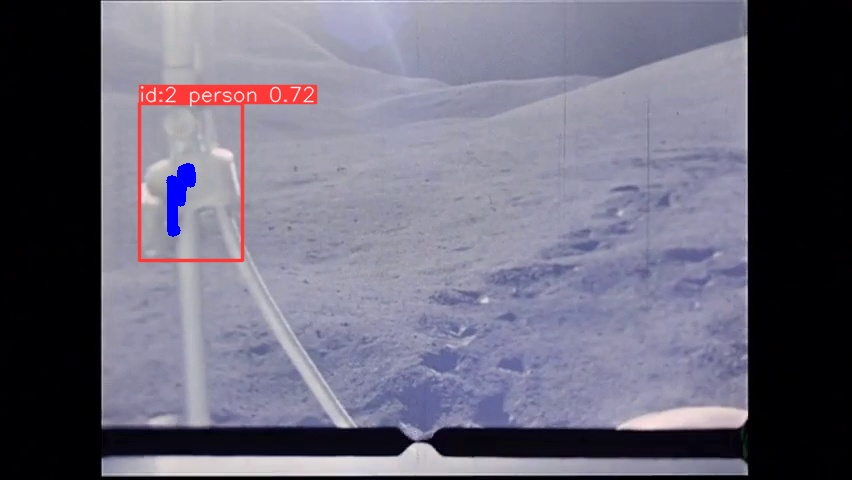
\includegraphics[width=12cm]{apollo15_10_1_1st_frame_400}\caption{Przyk\l adowa klatka z \protect\href{https://archive.org/download/Apollo15And1616mmOnboardFilm}{https://archive.org/download/Apollo15And1616mmOnboardFilm}.
\label{fig:R1}}
\end{figure}

\begin{figure}
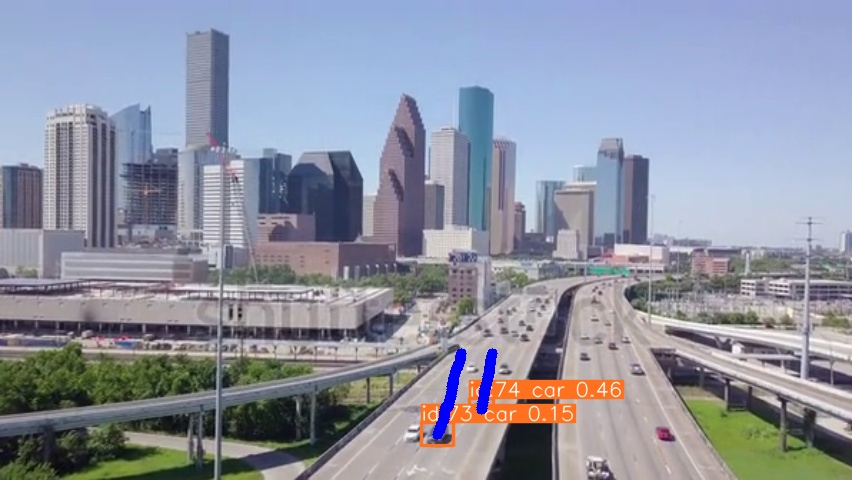
\includegraphics[width=12cm]{highway_drone_footage_frame_320}\caption{Przyk\l adowa klatka z \protect\href{https://shorturl.at/gALOU}{https://shorturl.at/gALOU}.}
\end{figure}

\begin{figure}
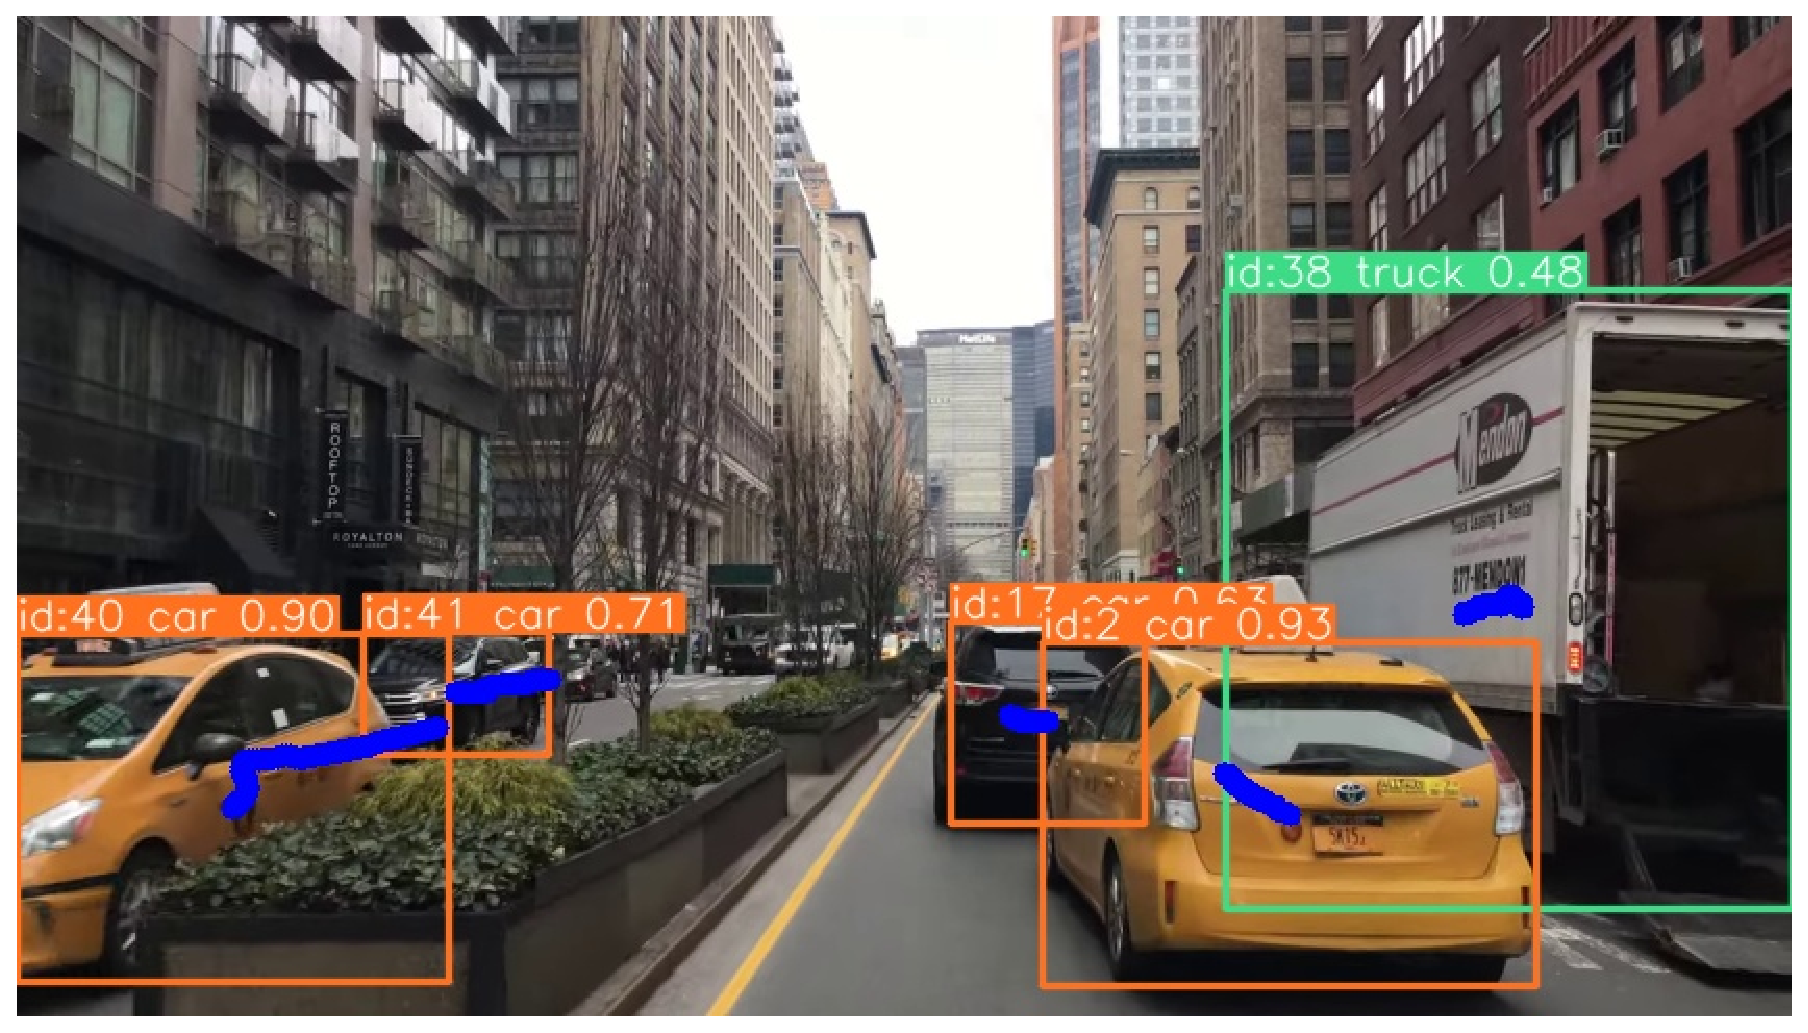
\includegraphics[width=12cm]{frame400}\caption{Przyk\l adowa klatka z \protect\href{https://youtu.be/7HaJArMDKgI?si=T0Bb3zOcz-YiOnMF}{https://youtu.be/7HaJArMDKgI?si=T0Bb3zOcz-YiOnMF}.}
\end{figure}

\begin{figure}
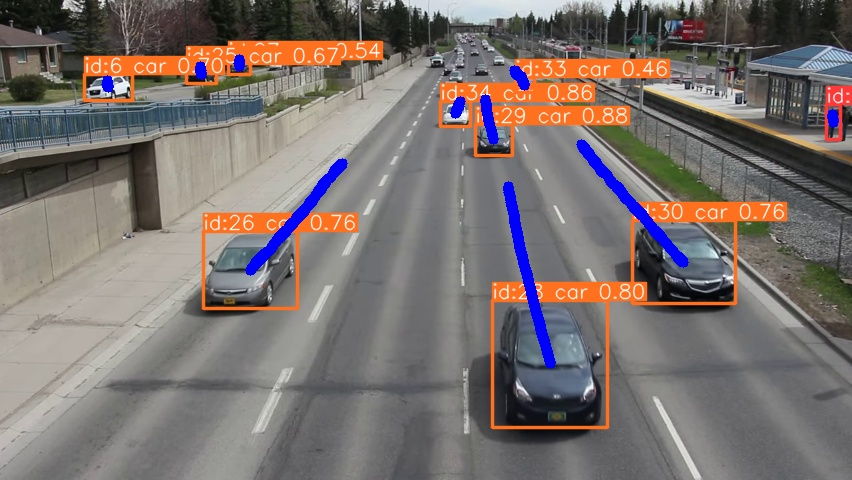
\includegraphics[width=12cm]{from_yt_2_frame_520}\caption{Przyk\l adowa klatka z \protect\href{https://youtu.be/Y1jTEyb3wiI?si=-gU51avblW5Qo-ij}{https://youtu.be/Y1jTEyb3wiI?si=-gU51avblW5Qo-ij}.}
\end{figure}

\begin{figure}
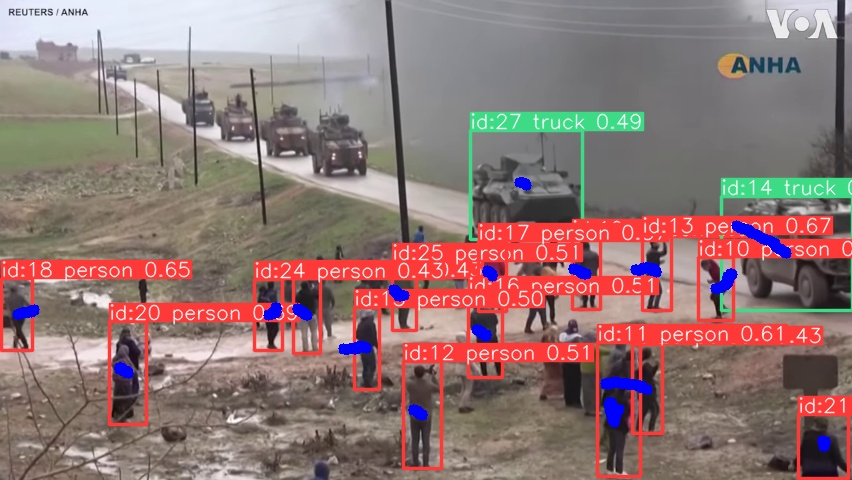
\includegraphics[width=12cm]{from_yt_3_frame_200}\caption{Przyk\l adowa klatka z \protect\href{https://youtu.be/jM2VrPE5kFg?si=RXfsB63fA58TuBSi}{https://youtu.be/jM2VrPE5kFg?si=RXfsB63fA58TuBSi}.}
\end{figure}

Uwagi:
\begin{enumerate}
\item Jak wida\'{c} na Rys. \ref{fig:R1}, model zdecydowanie nie widzia\l{}
wcze\'{s}niej danych z \l azik�w i b\l \k{e}dnie klasyfikuje jego
element jako osob\k{e} ...
\item Detekcja jest ograniczona rozdzielczo\'{s}ci\k{a}: obiekty o mniejszym
rozmiarze na klatce s\k{a} rzadziej wykrywane. Wykrywanie pojazd�w
w widoku ca\l kowicie z g�ry wydawa\l o si\k{e} r�wnie\.{z} dzia\l a\'{c}
gorzej.
\end{enumerate}

\end{document}
